\chapter{Implementation}\label{ch:Implementation}

This chapter describes the technical implementation of the forecasting pipeline, covering the technology stack, code structure, and the detailed implementation of each module---from data loading through model training to evaluation.


\section{Technology Stack}

The pipeline is implemented entirely in Python~3 using the libraries listed in Table~\ref{tab:tech_stack}. All experiments were run on a local machine; no GPU acceleration was required as the models are tree-based.

\begin{table}[H]
\centering
\caption{Technology stack and key libraries.}
\label{tab:tech_stack}
\begin{tabular}{@{}lll@{}}
\toprule
\textbf{Category} & \textbf{Library} & \textbf{Purpose} \\
\midrule
Data handling & \texttt{pandas}, \texttt{numpy} & DataFrame operations, numeric computation \\
Weather API & \texttt{requests} & HTTP requests to Open-Meteo \\
ML framework & \texttt{scikit-learn} & Linear Regression, Random Forest, scaling, CV \\
Gradient boosting & \texttt{xgboost} & XGBoost regressor \\
Gradient boosting & \texttt{catboost} & CatBoost regressor \\
Calendar features & \texttt{holidays} & Singapore public holiday detection \\
Configuration & \texttt{pyyaml} & YAML configuration parsing \\
Visualisation & \texttt{matplotlib}, \texttt{seaborn} & Plots and charts \\
Serialisation & \texttt{pickle} & Model persistence \\
\bottomrule
\end{tabular}
\end{table}


\section{Project Structure}

The codebase is organised into a modular directory structure:

\begin{lstlisting}[language={}, caption={Project directory structure.}, label={lst:project_structure}]
electricity-demand/
  configs/
    config.yaml          # Pipeline configuration
  data/
    ema_daily_demand.csv  # Input demand data
  src/
    data_loader.py        # Weather API + CSV loading
    preprocessing.py      # Feature engineering
    model.py              # Model definitions + PPSO
    trainer.py            # Training wrapper
    evaluator.py          # Metrics + plotting
    visualizer.py         # EDA visualisation
  main.py                 # Pipeline entry point
  results/                # Generated outputs
    plots/                # Visualisation images
    model_comparison.csv  # Leaderboard
    summary.yaml          # Summary statistics
\end{lstlisting}


\section{Data Loading Module}

The \texttt{data\_loader.py} module implements two data-loading functions and a merging function:

\subsection{Weather Data Retrieval}

The \texttt{fetch\_weather\_data()} function queries the Open-Meteo Archive API with the following parameters:
\begin{itemize}
    \item \textbf{Endpoint}: \texttt{https://archive-api.open-meteo.com/v1/archive}
    \item \textbf{Coordinates}: Latitude 1.3521, Longitude 103.8198 (Singapore)
    \item \textbf{Timezone}: \texttt{Asia/Singapore}
    \item \textbf{Variables}: \texttt{temperature\_2m\_mean}, \texttt{relative\_humidity\_2m\_mean}, \texttt{wind\_speed\_10m\_max}, \texttt{shortwave\_radiation\_sum}
\end{itemize}

The response JSON is parsed into a DataFrame with columns \texttt{date}, \texttt{temperature}, \texttt{humidity}, \texttt{wind\_speed}, and \texttt{solar\_radiation}. Any missing values are forward-filled to ensure continuity.

\subsection{Demand Data Loading}

The \texttt{load\_demand\_data()} function reads the EMA CSV file, validates the presence of the \texttt{demand\_mwh} column, and returns a sorted DataFrame.

\subsection{Data Merging}

The \texttt{load\_all\_data()} function orchestrates both data sources, performs an inner join on the \texttt{date} column, and validates that the merged dataset contains at least 31 observations.


\section{Preprocessing Module}\label{sec:preprocessing_impl}

The \texttt{DataPreprocessor} class in \texttt{preprocessing.py} applies three sequential feature engineering steps:

\subsection{Weather-Engineered Features}

The Comfort Climate Index (CCI) is computed when both temperature and humidity columns are present:
\begin{lstlisting}[language=Python, caption={CCI computation.}, label={lst:cci}]
df['cci'] = T + 0.55 * (1 - (RH / 100.0)) * (T - 14.5)
\end{lstlisting}

\subsection{Temporal Features}

Calendar-based features are extracted from the \texttt{date} column:
\begin{lstlisting}[language=Python, caption={Temporal feature extraction.}, label={lst:temporal}]
df['day_of_week'] = df['date'].dt.dayofweek   # 0=Mon, 6=Sun
df['month'] = df['date'].dt.month             # 1-12
df['is_weekend'] = df['day_of_week'].isin([5, 6]).astype(int)
df['is_holiday'] = df['date'].apply(
    lambda x: int(x in sg_holidays))
df['season'] = (df['month'] % 12 // 3 + 1).astype(int)
\end{lstlisting}

Public holidays are detected using the \texttt{holidays.SG()} class, which provides a comprehensive list of Singapore gazetted holidays for years 2023--2026.

\subsection{Lag and Rolling Features}

Autoregressive features are computed using shifted and rolling-window operations:
\begin{lstlisting}[language=Python, caption={Lag and rolling feature construction.}, label={lst:lag_rolling}]
for lag in [1, 7]:
    df[f'demand_lag_{lag}'] = df['demand_mwh'].shift(lag)

for window in [3, 7]:
    shifted = df['demand_mwh'].shift(1)
    df[f'demand_rolling_mean_{window}'] = (
        shifted.rolling(window=window).mean())
    df[f'demand_rolling_std_{window}'] = (
        shifted.rolling(window=window).std())
\end{lstlisting}

The \texttt{.shift(1)} applied before rolling ensures that only past data is used, preventing any look-ahead bias. Rows with NaN values introduced by lag and rolling operations are dropped at the end of the preprocessing step.


\section{Model Implementations}\label{sec:model_impl}

All models are instantiated through a factory function \texttt{create\_model(model\_type)}, which returns the appropriate model object.

\subsection{Linear Regression}

Scikit-learn's \texttt{LinearRegression} is used with default parameters. Input features are standardised using \texttt{StandardScaler} within the \texttt{ModelTrainer} wrapper.

\subsection{Random Forest}

\texttt{RandomForestRegressor} is configured with \texttt{random\_state=42} and \texttt{n\_jobs=-1} for reproducibility and parallel execution. Default hyperparameters are used, as the purpose is to establish a strong non-linear baseline.

\subsection{XGBoost}

\texttt{xgb.XGBRegressor} is configured with \texttt{random\_state=42} and \texttt{n\_jobs=-1}. Default hyperparameters are used.

\subsection{CatBoost (Default)}

\texttt{cb.CatBoostRegressor} is configured with the following categorical feature declarations:
\begin{lstlisting}[language=Python, caption={CatBoost categorical feature configuration.}, label={lst:catboost_cats}]
categorical_cols = ['season', 'day_of_week', 'month',
                    'is_weekend', 'is_holiday']
model = cb.CatBoostRegressor(
    random_state=42,
    cat_features=categorical_cols)
\end{lstlisting}

This allows CatBoost to use its native Target Statistics encoding rather than one-hot encoding, preserving ordinal information and reducing dimensionality.

\subsection{PPSO-Tuned Models}

The generic \texttt{PPSOTunedModel} class applies PPSO hyperparameter optimisation to any tree-based model (Random Forest, XGBoost, or CatBoost) under an identical optimisation budget, ensuring a fair comparison; \texttt{CatBoostPPSOModel} is retained as a thin backward-compatible subclass. Its core components are:

\subsubsection{PPSO Optimiser}

The \texttt{PPSO} class implements the optimisation loop described in Section~\ref{sec:ppso}:

\begin{enumerate}
    \item \textbf{Initialisation}: $N$ particles are uniformly sampled within the hyperparameter bounds. Phase angles $\theta$ are initialised uniformly in $[0, 2\pi]$.
    
    \item \textbf{Velocity update}: The PPSO velocity equation (Equation~\ref{eq:ppso_vel}) is applied element-wise:
    \begin{lstlisting}[language=Python, caption={PPSO velocity update implementation.}, label={lst:ppso_vel}]
cos_t = np.cos(Theta[i])
sin_t = np.sin(Theta[i])
term1 = (np.abs(cos_t)**2) * sin_t * (pbest_X[i] - X[i])
term2 = (np.abs(sin_t)**2) * cos_t * (gbest_X - X[i])
V[i] = term1 + term2
    \end{lstlisting}
    
    \item \textbf{Velocity clamping}: Maximum velocity is modulated by the cosine phasor term:
    \begin{lstlisting}[language=Python, caption={PPSO velocity clamping.}, label={lst:ppso_clamp}]
v_max = (np.abs(cos_t)**2) * (bounds[:, 1] - bounds[:, 0])
v_max = np.where(v_max < 1e-6,
    0.1 * (bounds[:, 1] - bounds[:, 0]), v_max)
V[i] = np.clip(V[i], -v_max, v_max)
    \end{lstlisting}
    
    \item \textbf{Position and phase update}:
    \begin{lstlisting}[language=Python, caption={PPSO position and phase angle update.}, label={lst:ppso_pos}]
X[i] = np.clip(X[i] + V[i], bounds[:, 0], bounds[:, 1])
Theta[i] = Theta[i] + np.abs(cos_t + sin_t) * (2 * np.pi)
    \end{lstlisting}
    
    \item \textbf{Early stopping}: If the global best fitness does not improve for 5 consecutive iterations, the loop terminates.
\end{enumerate}

\subsubsection{Objective Function}

The fitness of each particle is evaluated by training the candidate model (RF, XGBoost, or CatBoost) with the particle's decoded hyperparameters and computing the mean RMSE across 3-fold \texttt{TimeSeriesSplit} cross-validation:

\begin{lstlisting}[language=Python, caption={PPSO objective function (fitness evaluation).}, label={lst:ppso_obj}]
def _objective_function(self, params):
    hp = self._decode_params(params)  # model-specific bounds
    tscv = TimeSeriesSplit(n_splits=3)
    cv_rmse_scores = []
    for train_idx, val_idx in tscv.split(self.X_train):
        model = self._build_model(hp)  # RF / XGB / CatBoost
        model.fit(X_fold_train, y_fold_train)
        fold_rmse = np.sqrt(mean_squared_error(
            y_fold_val, model.predict(X_fold_val)))
        cv_rmse_scores.append(fold_rmse)
    return np.mean(cv_rmse_scores)
\end{lstlisting}

Each PPSO iteration therefore involves $N \times K = 15 \times 3 = 45$ training runs per tuned model. With early stopping limiting most runs to fewer than the maximum iterations, the total optimisation time remains practical.


\section{Training Wrapper}

The \texttt{ModelTrainer} class provides a unified interface for all models:

\begin{itemize}
    \item \textbf{Scaling}: Optional \texttt{StandardScaler} is applied for models that benefit from normalised features (Linear Regression). Tree-based models receive unscaled data.
    \item \textbf{Training}: The \texttt{fit()} method delegates to the model's own \texttt{fit()} method, passing any additional keyword arguments (e.g.\ \texttt{param\_bounds} for CatBoost-PPSO).
    \item \textbf{Prediction}: The \texttt{predict()} method applies the same scaling transform (if any) before calling the model's \texttt{predict()}.
    \item \textbf{Persistence}: Trained models, scalers, and feature names are serialised to disk using \texttt{pickle}.
\end{itemize}


\section{Evaluation Module}

The \texttt{RegressionEvaluator} class computes all six metrics described in Section~\ref{sec:eval_metrics}. The implementation uses \texttt{scikit-learn}'s \texttt{mean\_absolute\_error}, \texttt{mean\_squared\_error}, and \texttt{r2\_score}, supplemented by custom implementations for MAPE, RAE, and WI:

\begin{lstlisting}[language=Python, caption={Custom metric implementations.}, label={lst:metrics}]
epsilon = np.finfo(np.float64).eps
mape = np.mean(np.abs((y_true - y_pred) /
               (y_true + epsilon))) * 100
rae = np.sum(np.abs(y_true - y_pred)) / (
      np.sum(np.abs(y_true - np.mean(y_true))) + epsilon)
wi_num = np.sum((y_pred - y_true)**2)
wi_den = np.sum((np.abs(y_pred - np.mean(y_true)) +
         np.abs(y_true - np.mean(y_true)))**2)
wi = 1 - (wi_num / (wi_den + epsilon))
\end{lstlisting}

A machine epsilon (\texttt{eps}) is added to denominators to prevent division-by-zero errors.


\section{Pipeline Orchestration}

The \texttt{main.py} script orchestrates the entire pipeline in seven sequential steps:

\begin{enumerate}
    \item Load configuration from \texttt{configs/config.yaml}.
    \item Load and merge weather + demand data.
    \item Run preprocessing and feature engineering.
    \item Execute EDA visualisation.
    \item Perform chronological train/test split.
    \item Train all models (including PPSO optimisation for every tree-based model: RF-PPSO, XGB-PPSO, CatBoost-PPSO).
    \item Evaluate all models, generate leaderboard, and save results.
\end{enumerate}

The entire pipeline is executed via a single command: \texttt{python main.py}.


\section{Interactive Forecasting Dashboard}\label{sec:dashboard}

Beyond the offline experimentation pipeline, a lightweight web-based portal was developed to make the trained model accessible to non-technical stakeholders. The portal consists of two pages: a \emph{History Report} page for exploring past demand and the model's retrospective accuracy over a user-selected period, and a \emph{Demand Trends} page that produces forward-looking demand outlooks by combining the trained CatBoost-PPSO model with live weather forecasts from the Open-Meteo API \parencite{openmeteo2025api}.

\subsection{Architecture}

The dashboard follows a conventional two-tier client--server architecture:

\begin{itemize}
    \item \textbf{Backend (FastAPI, Python)}: A thin REST service that loads the serialised \texttt{catboost\_ppso\_model.pkl} at start-up and exposes four endpoints: \texttt{/api/summary} (model metadata and test-set metrics), \texttt{/api/range} (historical demand, per-day model predictions, and user-friendly statistics for a selected period of at least 30 days), \texttt{/api/predict} (single-date forecast), and \texttt{/api/forecast} (multi-day forward outlooks driven by Open-Meteo weather forecasts).
    \item \textbf{Frontend (React + Vite)}: A single-page application with tab-based navigation between the two pages. Charts are drawn with the Recharts library, and the layout uses a card-based grid with a restrained colour palette to keep the interface clean and legible. Technical metric names are translated into plain language for general users (e.g.\ ``forecast accuracy'' in place of $R^2$/MAPE, and human-readable feature names such as ``Yesterday's demand'' in place of \texttt{demand\_lag\_1}).
\end{itemize}

\subsection{Weather Forecast Integration (Open-Meteo)}

The Demand Trends page requires weather values for future dates, which are obtained from two Open-Meteo services \parencite{openmeteo2025api}:

\begin{itemize}
    \item \textbf{Short/medium range (up to 16 days)}: the standard forecast endpoint (\texttt{api.open-meteo.com/v1/forecast}) is queried with \texttt{forecast\_days=16} and \texttt{timezone=Asia/Singapore}, retrieving daily maximum/minimum temperature, precipitation, humidity, wind speed, and solar radiation. The user may choose between the default \texttt{best\_match} model selection and the European \texttt{ecmwf\_ifs025} model.
    \item \textbf{Long range (monthly and seasonal outlooks, up to 6 months)}: the climate endpoint (\texttt{climate-api.open-meteo.com/v1/climate}) provides seasonal-scale daily estimates. Where neither service covers a requested day, the monthly climatology of the historical dataset is used as a fallback.
\end{itemize}

The portal explicitly communicates the accuracy characteristics of numerical weather prediction to the user: forecasts for the first 1--3 days are highly reliable (approximately 85--95\% for temperature, wind, and pressure), days 4--7 remain useful for identifying trends (approximately 70--80\%), while days 8--16 are indicative only (approximately 50--60\%) and are best interpreted as general tendencies rather than precise daily values. Monthly and seasonal outlooks derived from climate models are presented as smoothed trends rather than day-level predictions.

\subsection{Recursive Demand Prediction}

The trained model requires the full 16-feature vector described in Section~\ref{sec:preprocessing_impl}, including autoregressive lag and rolling features. For future dates these are not observable, so the backend performs \emph{recursive} (iterated) forecasting: starting from the last observed day in the dataset, the model predicts one day at a time, and each prediction is appended to the demand buffer used to compute the lag and rolling features of subsequent days. Temporal features are derived deterministically from each date (including the Singapore holiday calendar), and weather features are taken from the Open-Meteo services described above.

It should be noted that this deployment strategy compounds two sources of uncertainty --- weather forecast error and accumulated autoregressive error --- and therefore yields lower accuracy than the retrospective evaluation reported in Chapter~\ref{ch:Evaluation}, degrading progressively with the forecast horizon. This trade-off is acceptable for the portal's purpose of communicating expected demand trends; the research contribution of this project remains the retrospective comparative study of how weather variables influence electricity demand, for which the evaluation methodology in Chapter~\ref{ch:Evaluation} is unaffected.

\subsection{Dashboard Interface}

The \emph{History Report} page is organised into four areas: (i) a period selector (date range, month, or year, validated to cover at least 30 days), (ii) summary cards showing average daily use, busiest and quietest days, and forecast accuracy for the selected period, (iii) a time-series chart of actual versus model-predicted demand, and (iv) supporting charts showing average demand by day of week and the model's most influential factors.

The \emph{Demand Trends} page offers three outlook modes --- the next 7 or 16 days, a calendar month, or a season (quarter), limited to 6 months ahead --- together with a weather-model selector, a confidence banner that states the expected reliability of the current horizon, the projected demand series (smoothed for long-range outlooks), and the underlying temperature forecast.

\begin{figure}[H]
    \centering
    % TODO: Replace the placeholder rule below with the actual dashboard screenshot, e.g.:
    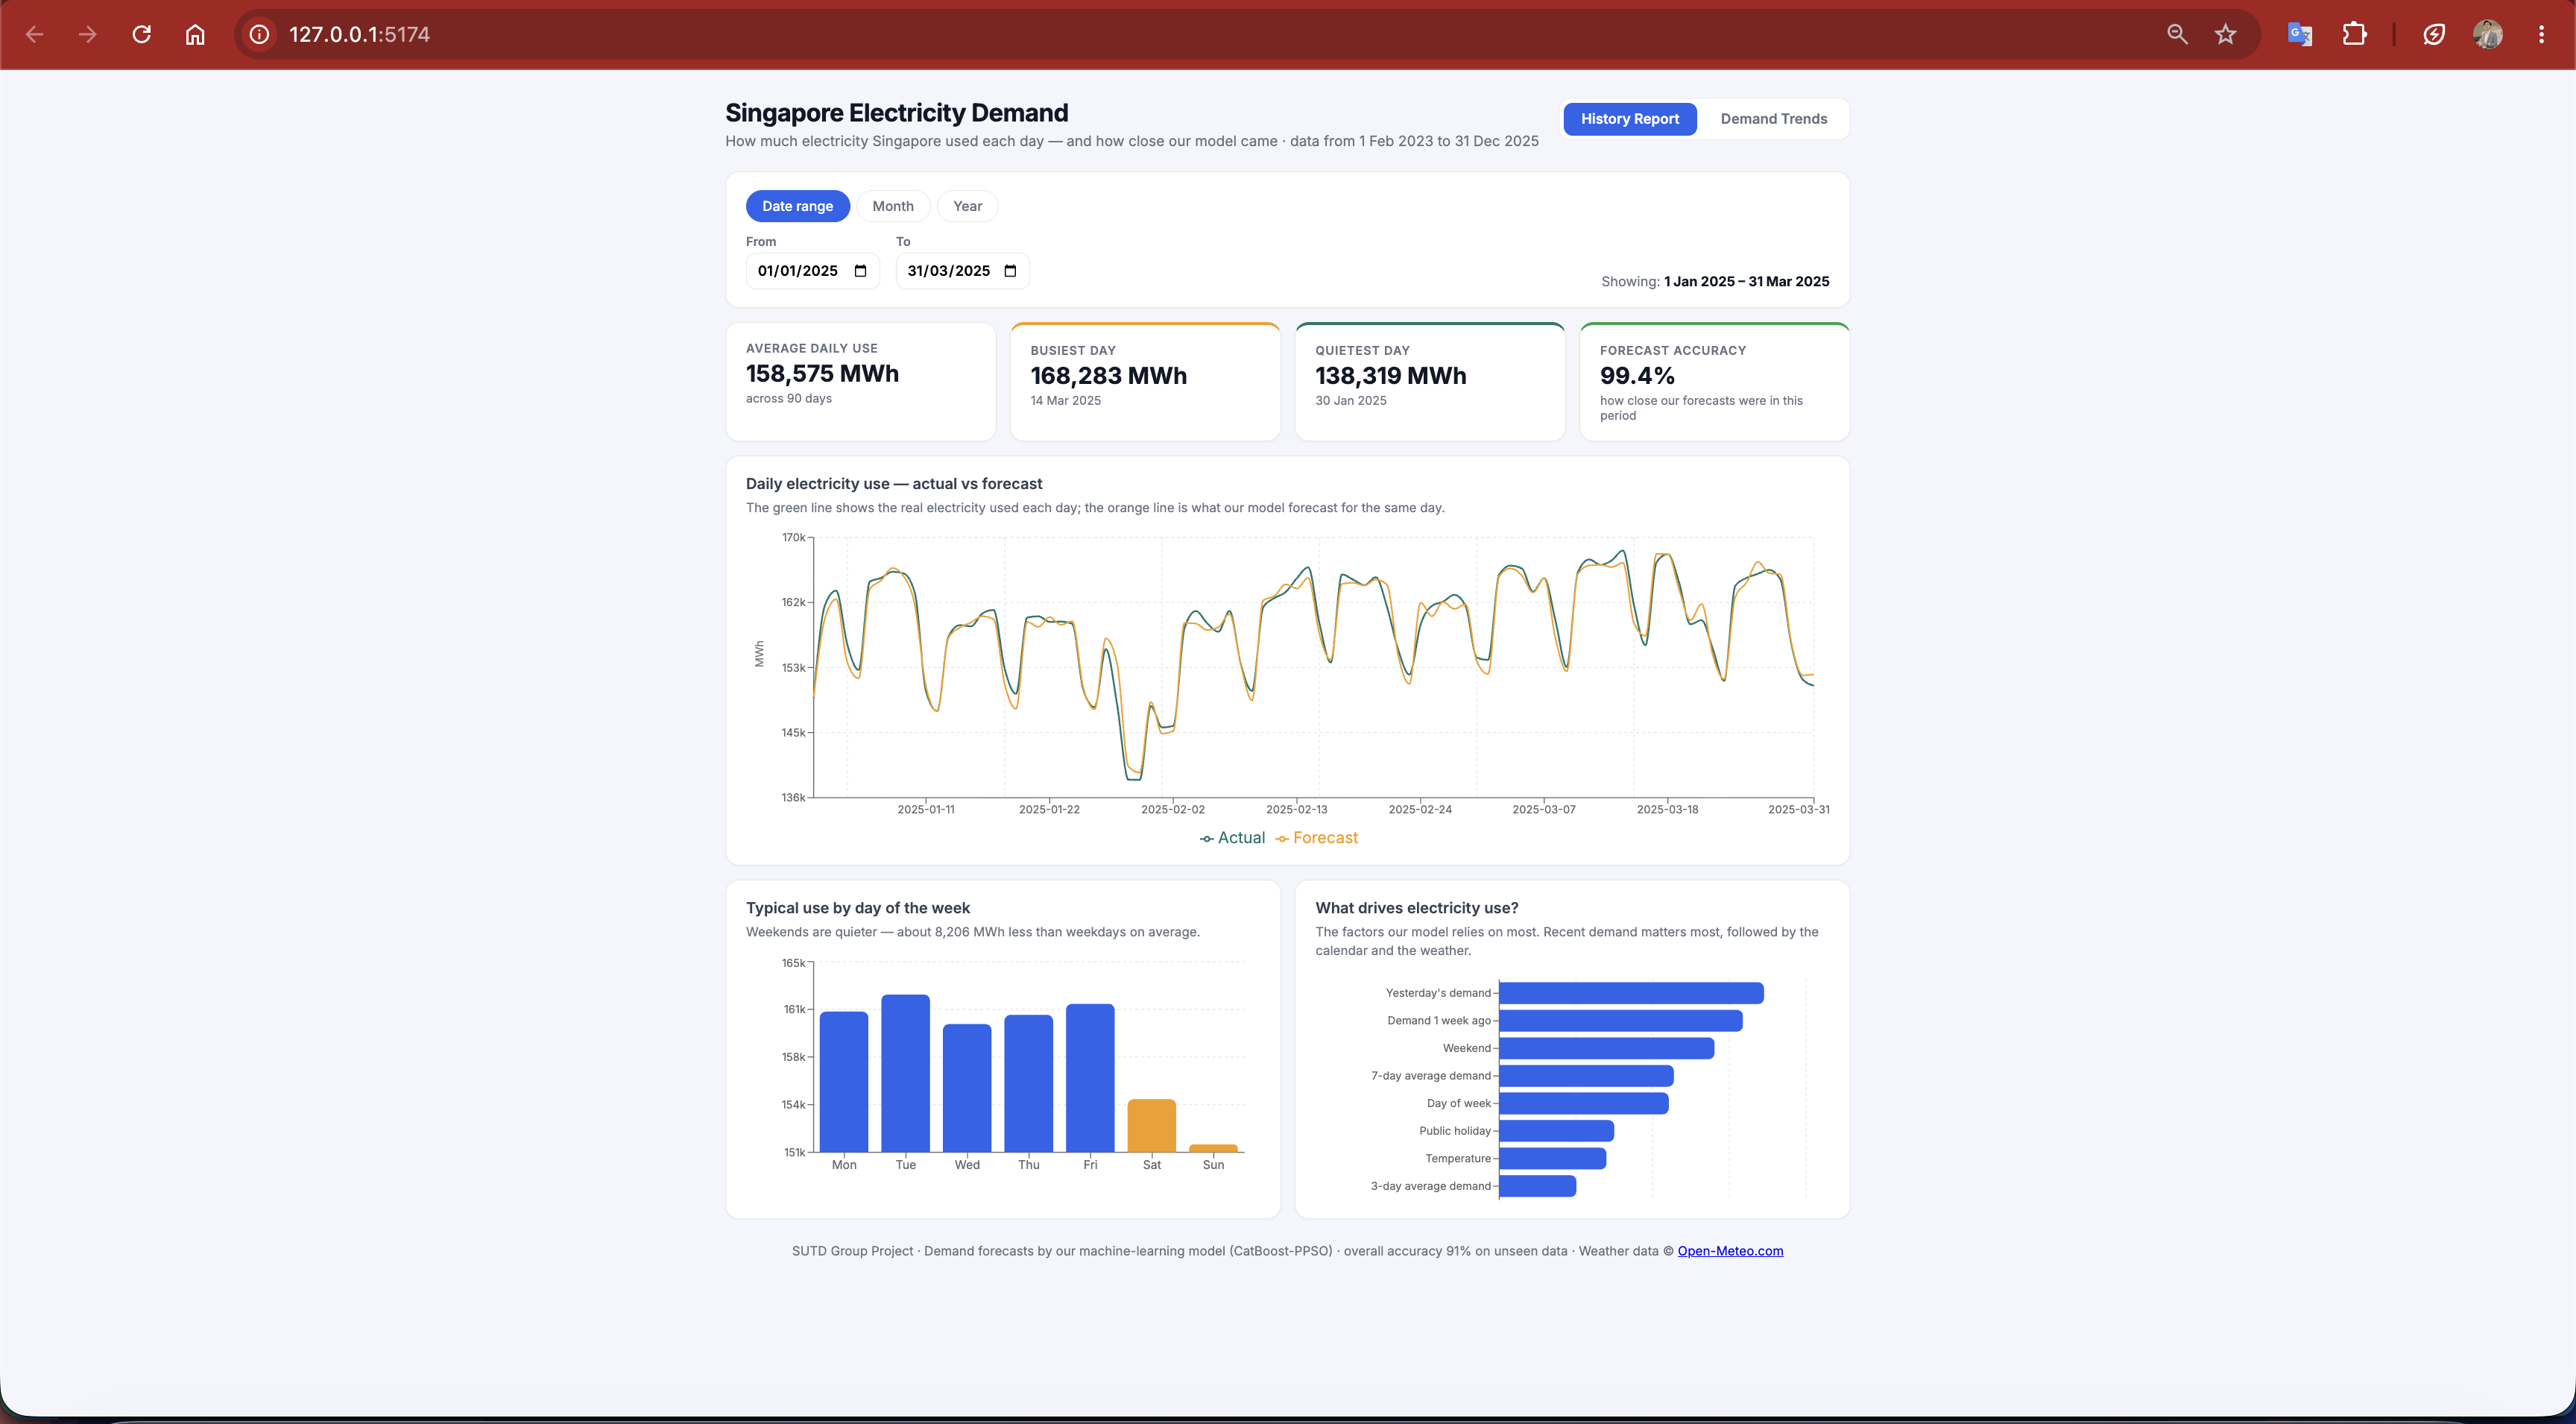
\includegraphics[width=0.95\textwidth]{impl/images/dashboard_history.png}
    % \fbox{\parbox[c][7cm][c]{0.9\textwidth}{\centering \emph{Placeholder --- insert History Report page screenshot here}\\ \texttt{impl/images/dashboard\_history.png}}}
    \caption{History Report page of the dashboard: period selector, summary cards, actual versus predicted demand, and supporting charts for the selected period.}
    \label{fig:dashboard_overview}
\end{figure}

\begin{figure}[H]
    \centering
    % TODO: Replace the placeholder rule below with the actual trends page screenshot, e.g.:
    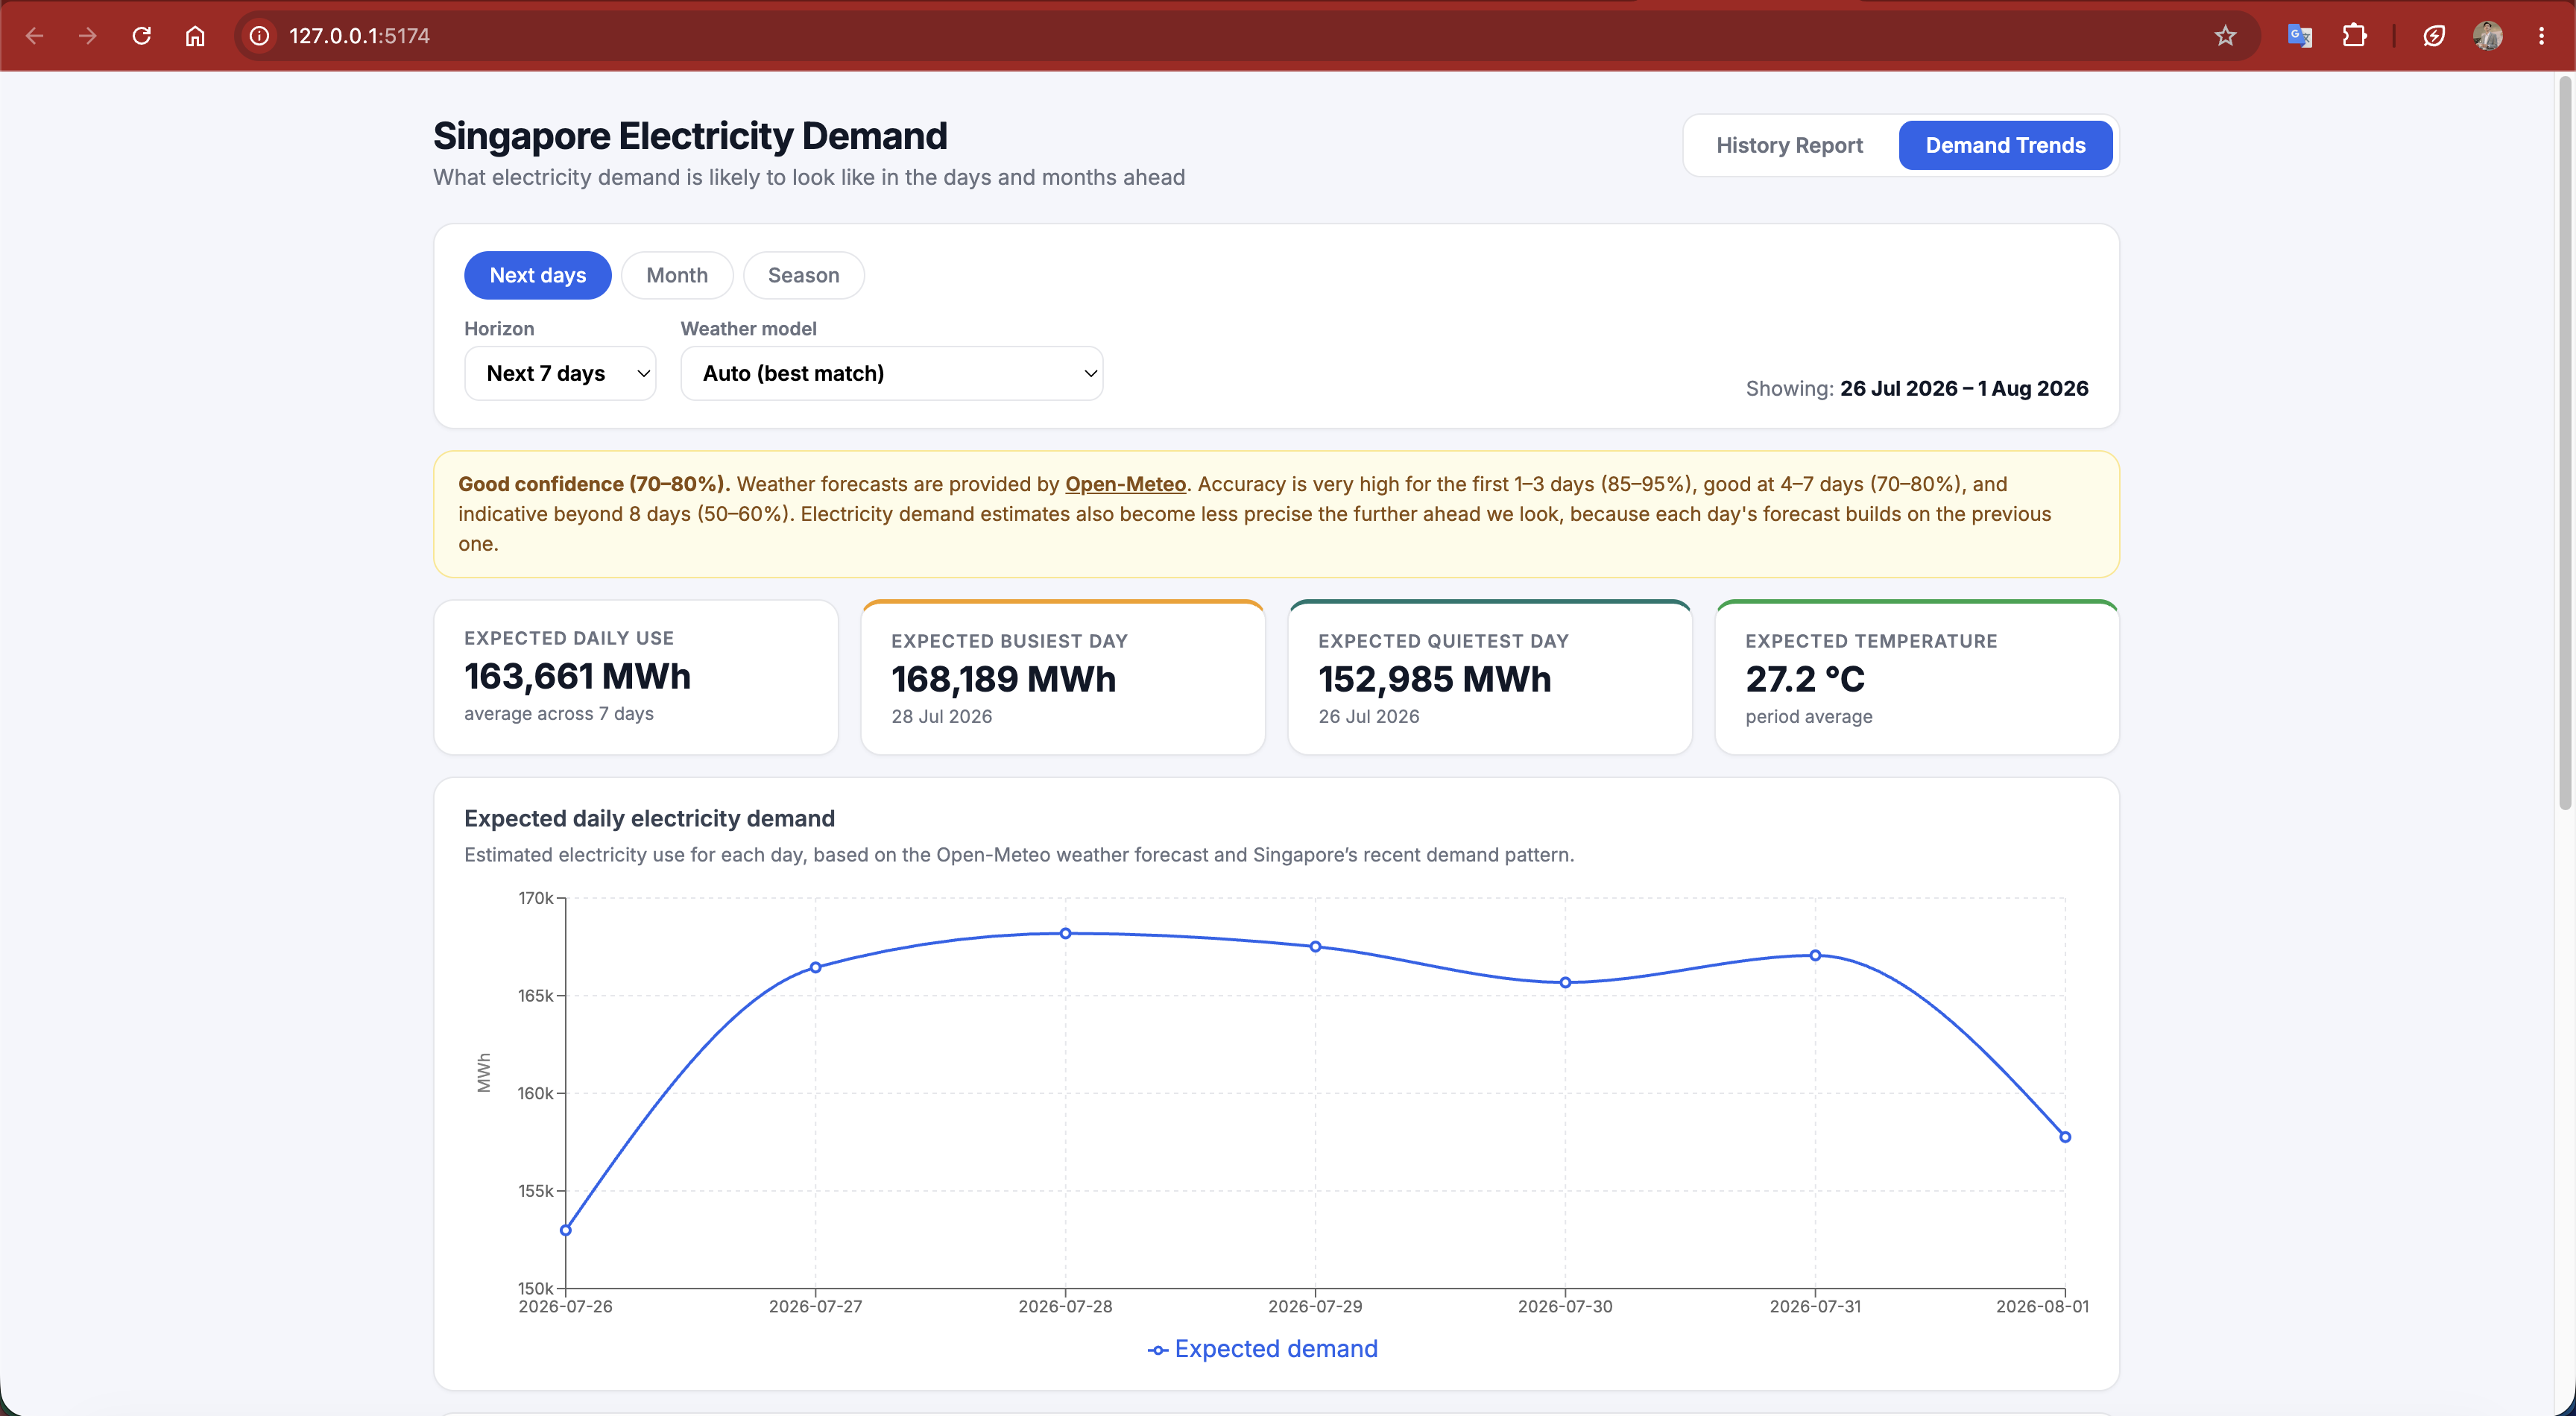
\includegraphics[width=0.95\textwidth]{impl/images/dashboard_trends.png}
    % \fbox{\parbox[c][7cm][c]{0.9\textwidth}{\centering \emph{Placeholder --- insert Demand Trends page screenshot here}\\ \texttt{impl/images/dashboard\_trends.png}}}
    \caption{Demand Trends page of the dashboard: forward-looking demand outlook driven by Open-Meteo weather forecasts, with an explicit confidence banner reflecting the forecast horizon.}
    \label{fig:dashboard_prediction}
\end{figure}


\section{Conclusions}

This chapter has described the implementation of each module in the forecasting pipeline. The code follows a modular design that separates concerns (data loading, preprocessing, modelling, evaluation) and uses a central configuration file for reproducibility. The PPSO implementation closely follows the mathematical formulation of Ghasemi et al.\ \parencite{ghasemi2019ppso}, with adaptations for tree-model hyperparameter tuning and time-series cross-validation, applied uniformly to Random Forest, XGBoost, and CatBoost. In addition, an interactive web dashboard was implemented to expose the trained CatBoost-PPSO model through a simple date-based prediction interface. The following chapter presents the experimental results and comparative evaluation of all model configurations.
